\section{Was wird f�r die App Programmierung ben�tigt}
\index{App Inventor}
Es gibt eine ganze Reihe von M�glichkeiten, ein Android App zu programmieren. Neben Software, die er erlaubt, offline zu programmieren, gibt es von Google eine Online-Plattform, welche es erlaubt, ohne Programmierkenntnisse ein App zu erstellen. Diese M�glichkeit ist jedoch beim Umfang der M�glichkeiten beschr�nkt und l�uft auf einer Beta-Phase. F�r eine Nutzung von Googles \href{http://beta.appinventor.mit.edu/}{App Inventor}\footnote{offizielle Website: \url{http://beta.appinventor.mit.edu/}} ist ein Google Account notwendig.\\
Ein Screenshot der Weboberfl�che  (\refTC{fig:App_Inventor}) sowie der Textbausteine (\refTC{fig:Screenshot_AppInventor_Block}) sind im Anhang zu finden.

Da wir in den ersten beiden Studienjahren uns einige Java-Kenntnisse aneignen konnten, wird auf die Nutzung und das Austesten von Googles \href{http://beta.appinventor.mit.edu/}{App Inventor} verzichtet.\\ 
Die einfachste Weise ist die Nutzung der uns zum Teil bereits bekannten Frameworks. Nachfolgend werden alle benutzten Frameworks kurz erl�utert.



%-------------------------------------------------------------------------------------
\newpage
\subsection{Eclipse (IDE)} \index{Eclipse}
\href{http://www.eclipse.org}{Eclipse} \footnote{offizielle Website: \url{http://www.eclipse.org}} (vom englischen eclipse = Sonnenfinsternis hergeleitet) ist ein open-source Programmierwerkzeug. Zu Beginn wurde Eclipse als eine Entwiklungsumgebung f�r Java entwickelt. Im Laufe der Zeit hat sich Eclipse weiterentwickelt und durch die M�glichkeit der Skalierbarkeit wurde vom Java-Programmiertool ein Werkzeug, welches f�r viele Entwicklungsaufgaben eingesetzt werden kann. Die grosse Community und der modulare Aufbau, welche die Weiterentwicklung vom Modulen und Plugins  immer vorantreiben, haben aus diesem Tool ein m�chtiges Tool gemacht, welches sich f�r den Entwickler individuell zuschneiden l�sst.
Es gibt f�r Eclipse mittlerweile open-souce sowie auch kommerzielle Erweiterungen.
Eclipse selbst basiert auf Java-Technik, seit Version 3.0 auf einem sogenannten OSGi-Framework namens Equinox.\\
Speziell f�r die Entwicklung von Android Applikationen
existiert das ADT (Android Development Tools) Plug-in. Dieses Plug-in erweitert den
Funktionsumfang von Eclipse und erm�glicht somit ein einfaches Entwickeln von Android
Projekten.
Eclipse wurde als Grundwerkzeug f�r die App-Programmierung benutzt. In den ersten beiden Studienjahren haben wir mit Eclipse Java-Applikationen entwickelt.\\ \\
Quelle: \cite{wiki_eclipse} 
\begin{figure}[h]
\centering
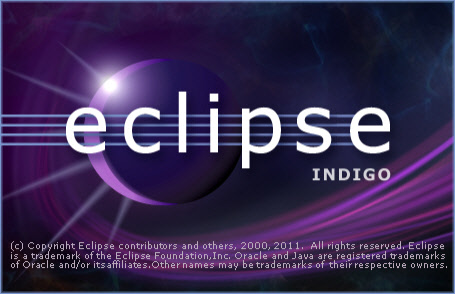
\includegraphics[height=5cm]{eclipse_logo.png} \\
\caption{Logo Eclipse IDE}
\label{Logo_Eclipse IDE}
\end{figure}

%-------------------------------------------------------------------------------------
\newpage
\subsection{Android SDK Plugin  for Eclipse}
\index{Android SDK}
\index{AVD Manager}
Das Android Software Development Kit (SDK) \footnote{\url{http://developer.android.com/sdk/index.html}} \cite{andoid_sdk_eclipse} ist ein Plugin f�r Eclipse IDE welches als m�chtige, integrierte Entwicklungsumgebung konzipiert wurde, um Android Applikationen zu entwickeln.\\
Will man beginnen, Android Apps zu programmieren, kommt man um das Android SDK nicht herum.\\
Die Android SDK gibt es f�r Windows, Mac OS X sowie Linux Plattformen.\\
Um Android SDK nutzen zu k�nnen, ist die Java SDK (Software Development Kit) unabdingbar. Diese ist je nach Betriebssystem bereits vorinstalliert oder kann nachtr�glich heruntergeladen und installierte werden.\\
Im Android SDK integriert ist der AVD Manager (Android Virtual Device Manager). Dieser erm�glicht das Testen der App in einer virtuellen Umgebung. Das Betriebssystem, die Speicherm�glichkeiten sowie das Telefon k�nnen beliebig ge�ndert werden.\\
\\
\\
\begin{figure}[h]
\centering
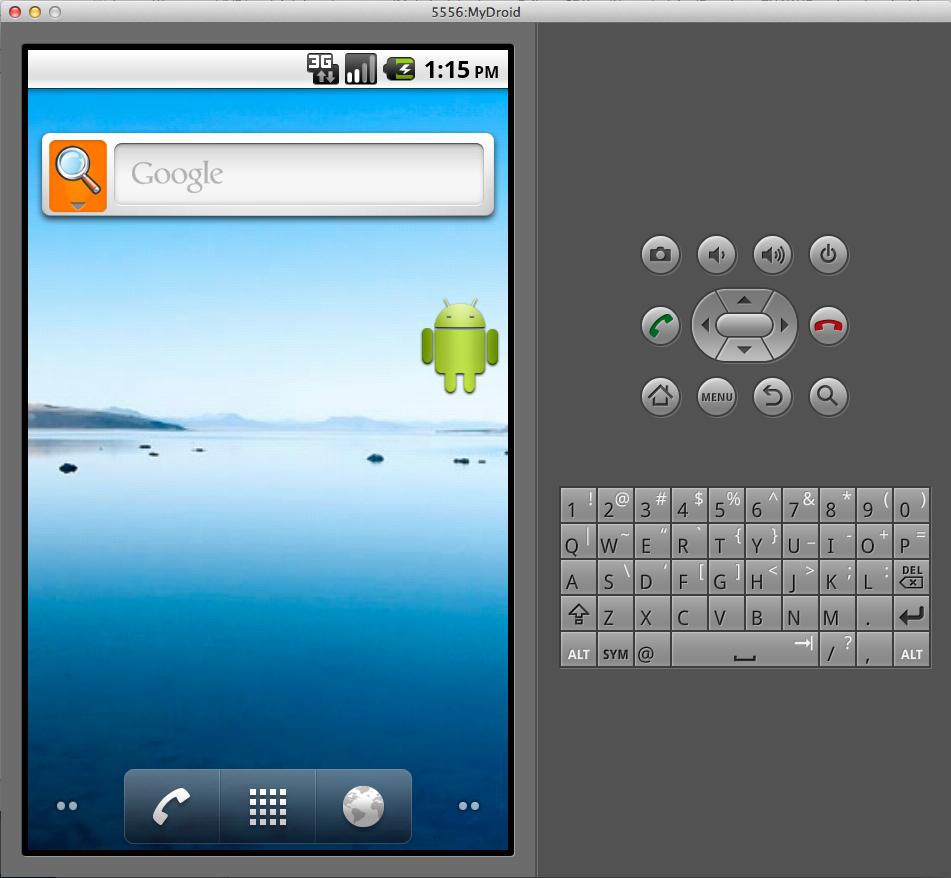
\includegraphics[height=7.5cm]{AVD_Manager.png} \\
\caption{Beispiel AVD Manager}
\label{Bsp_AVD_Manager}
\end{figure}

%-------------------------------------------------------------------------------------
\newpage
\subsection{Testing}
Da die Zeit f�r dieses Projekt nicht ausreicht f�r ein ausgiebiges Testen mit JUnit- und JMock-Klassen, haben wir uns auf ein Testing beschr�nkt auf das Live-Testing.
Zur Auswahl standen:
\begin{itemize}
\item Galaxy Nexus, Version 4.0.1
\item HTC Desire HD, Version 2.3.5
\item virtuelle Maschine, welche in Eclipse integriert ist und sich wahlweise die Android Version, aber auch Telefontyp �ndern l�sst
\end{itemize}
